\documentclass[12pt,a4paper]{article}

\usepackage[T2A]{fontenc}
\usepackage[utf8]{inputenc}
\usepackage[english,russian]{babel}
\usepackage{indentfirst}
\usepackage{hyperref}
\usepackage{amsmath,amsthm,amstext,amssymb,amscd}
\usepackage{mathtools}
\usepackage{mathrsfs}
\usepackage{graphicx}
\usepackage{caption}
\usepackage{subcaption}

\newcommand*\Laplace{\mathop{}\!\mathbin\bigtriangleup}

\title{Распределение тепла в пластине \\ Метод Якоби}
\author{Игорь Степанов, ФРТК, 213}

\begin{document}

\maketitle
\hrulefill

\section{Постановка задачи}
\label{sec:problem}

Для уравнения 

\begin{equation}
	\Laplace U = -f(x, y), f(x, y) = -2(x^2+y^2) + 2(x+y), U|_{\delta\Omega} = 0
\end{equation}

в области $\Omega = [0,1]\cap[0,1]$ найти распределение тепла в пластине численно. При решении СЛАУ использовать итерационный метод Якоби для равномерной сетки с шагом по обоим направлениям $h \in \{10^{-1}, 10^{-2}, \dots, 10^{-7}\} $ \par

Точное решение имеет вид:

\begin{equation}
	U(x, y) = xy(1-x)(1-y)
\end{equation}

\section{Метод Якоби}
\label{sec:yacobi}

Для метода Якоби используется разностная схема: 
\begin{equation}
	U^{(k+1)}_{i, j} = \frac{1}{4} \left(U^{(k)}_{i - 1, j} + U^{(k)}_{i + 1, j} + U^{(k)}_{i, j - 1} + U^{(k)}_{i, j + 1} - h^2 f_{i, j} \right)
\end{equation}

\section{Результат}
\label{sec:theory}

\begin{tabular}{|l|l|l|l|}

\hline
Шаг h & Точность $\varepsilon$ & Кол-во итераций N & Ошибка err \\
\hline
0.1 & 0.1 & 1 & 0.05771015319824219 \\
0.01 & 0.01 & 1977 & 0.009993698168278047 \\
0.001 & 0.001 & - & - \\
0.0001 & 0.0001 & - & - \\
\hline

\end{tabular}


\begin{figure}
	\centering
	\begin{subfigure}{\textwidth}
		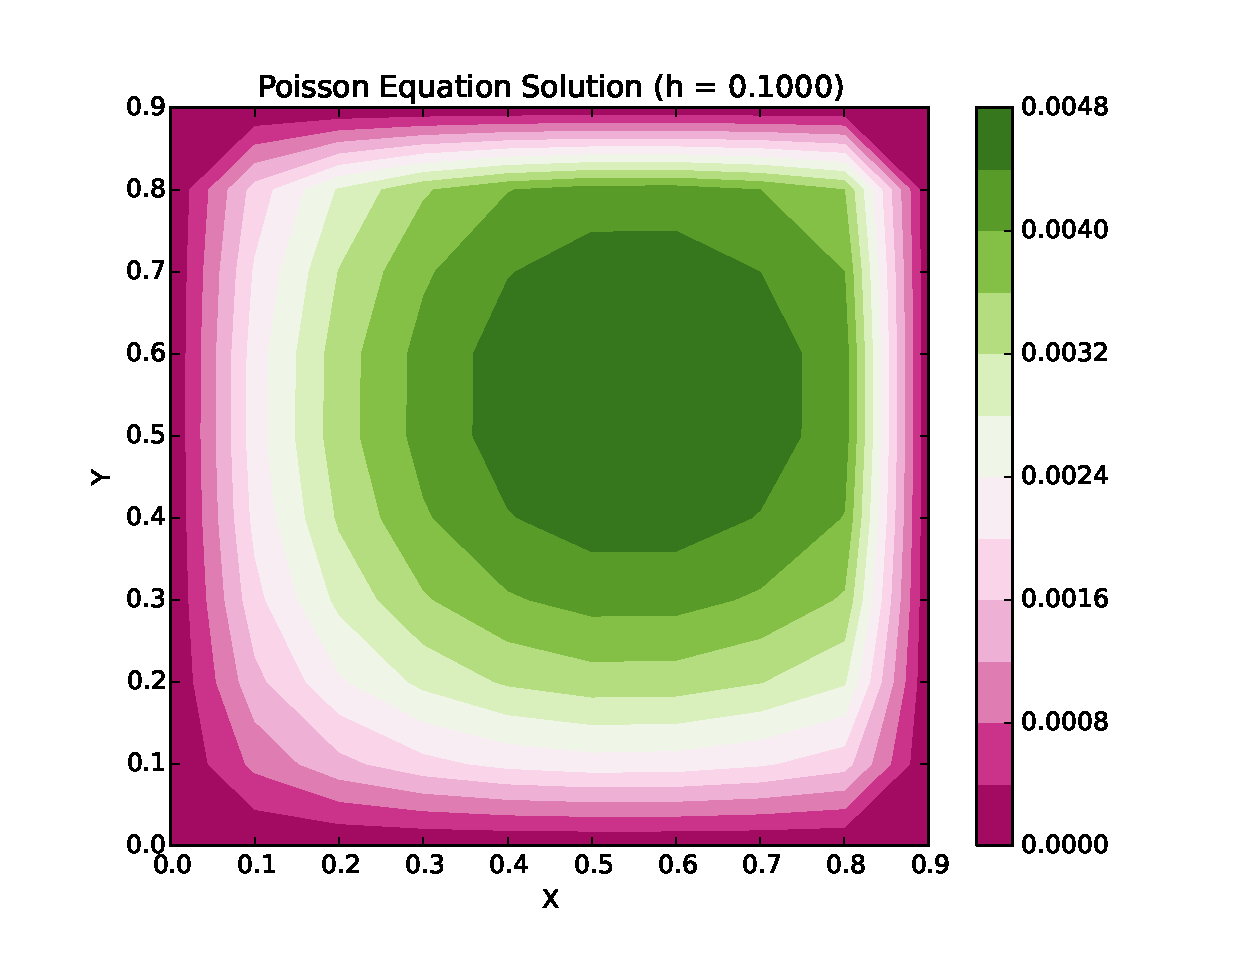
\includegraphics{1_u.eps}
		\caption{Метод Якоби}\label{fig:u0.1}
	\end{subfigure}
	\begin{subfigure}{\textwidth}
		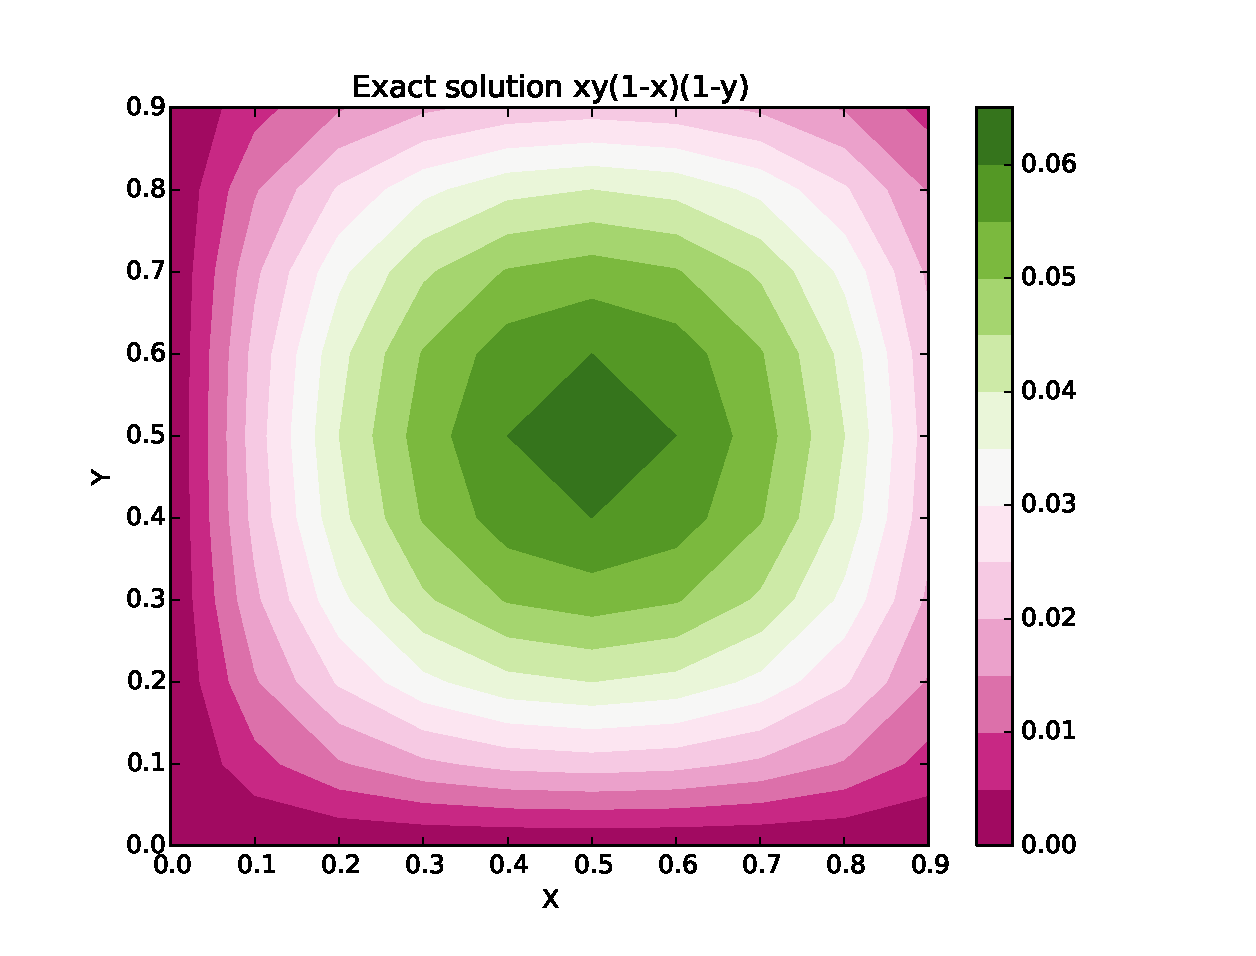
\includegraphics{1_exact.eps}
		\caption{Точное решение}\label{fig:e0.1}
	\end{subfigure}
	\caption{Шаг $h=0.1$}\label{fig:e0.1}
\end{figure}

\begin{figure}
	\centering
	\begin{subfigure}{\textwidth}
		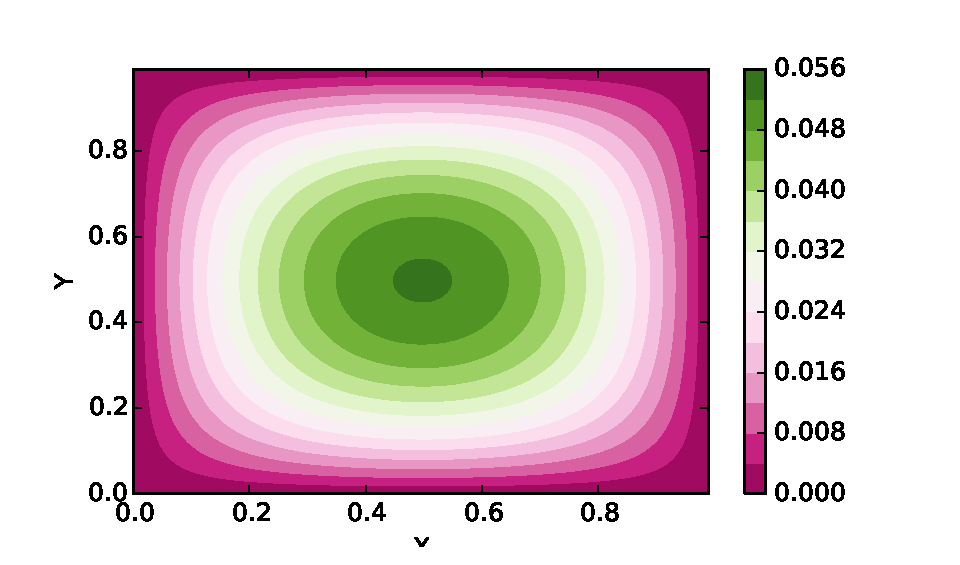
\includegraphics{01_u.eps}
		\caption{Метод Якоби}\label{fig:u0.01}
	\end{subfigure}
	\begin{subfigure}{\textwidth}
		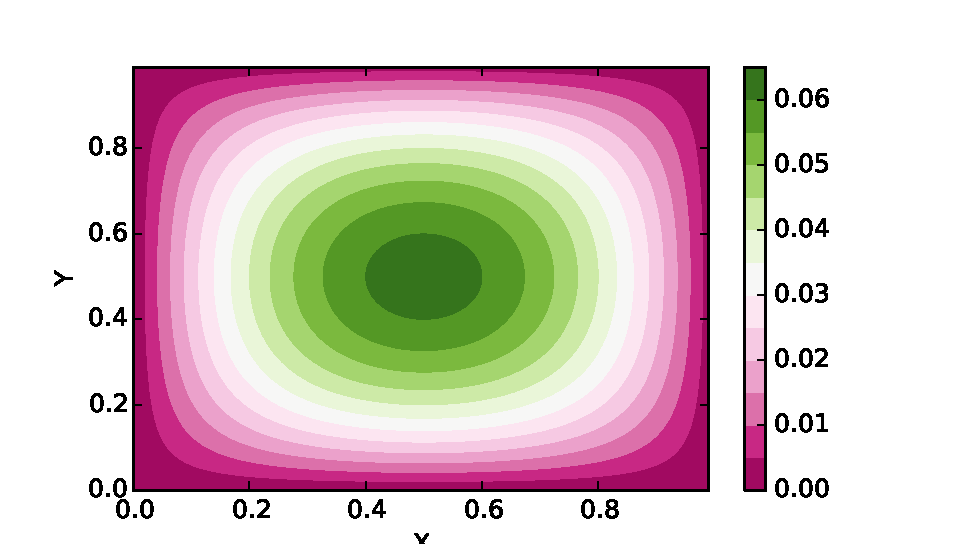
\includegraphics{01_exact.eps}
		\caption{Точное решение}\label{fig:e0.01}
	\end{subfigure}
	\caption{Шаг $h=0.01$}\label{fig:e0.01}
\end{figure}

\section{Заключение}
\label{sec:summary}

Из графиков видно, что метод Якоби хорошо приближает к точному решению. В моей имплиментации использовался язык программирования Python с библиотекой MatPlotLib для построения графиков. В программе можно сохранить результат в файл на диск, напечатать в терминале или же построить графики для самого метода и для точного решения задачи. \par
Однако данный метод слишком ресурсоемкий, т.к. для шагов $h=0.001$ и $h=0.0001$ результаты получить более чем за 12 часов не удалось. Возможно проблема в неоптимальном алгоритме и нехватки мощности компьютера. Так например для шага $h=0.001$ требовалось более 3 Гб оперативной памяти.

% На Рис.~\ref{fig:fig2} показано решение исходной задачи (раздел~\ref{sec:problem}) двухстадийным явным методом Рунге-Кутты (формула \ref{eq:runge-x2}). Сравнивая с Рис.~\ref{fig:fig1}, видно, что решения практически повторяют друг друга, а так как среде Matlab можно доверять, то и наше решение будет верным. \par
% При уменьшении шага примерно до $h \simeq 0.1 $ двухстадийный метод становится непригодным для использования, а Matlab продолжает считать верно. \par


\end{document}
